%%% Local Variables:
%%% mode: latex
%%% TeX-master: "../doc"
%%% coding: utf-8
%%% End:
% !TEX TS-program = pdflatexmk
% !TEX encoding = UTF-8 Unicode
% !TEX root = ../doc.tex

\section{From Artificial Intelligence to Large Language Models}

The term \textbf{Artificial Intelligence} (AI) refers broadly to the field of computer science concerned with building systems that can perform tasks which would ordinarily require human intelligence, such as recognizing patterns, drawing inferences, or generating language \cite{stoffelbauer_how_2023}. Within this field, \textbf{Machine Learning} (ML) denotes a subset of approaches in which systems are not explicitly programmed with rules but instead learn to perform tasks by identifying statistical regularities in data. \textbf{Deep Learning} is a further specialization within machine learning that relies on artificial neural networks composed of many layers, enabling systems to learn highly abstract representations from raw input such as text, images, or audio.

\textbf{Large Language Models} (LLMs) are a class of deep learning systems trained on vast corpora of text with the objective of modelling the probability distribution over sequences of tokens. In practical terms, this means that an LLM learns to predict, given a preceding sequence of words, which words are most likely to follow. Through training on text at an enormous scale, LLMs acquire broad linguistic competence as well as a form of implicit factual and procedural knowledge encoded in their parameters.

\section{The LLM Pipeline}

Understanding how LLMs are built and deployed is relevant context for evaluating their outputs and the role of explainability. The life-cycle of an LLM can be divided into three phases: pre-deployment, inference, and post-deployment.

\subsection{Pre-Deployment: Training and Preparation}

The foundation of any LLM is a base model trained on a large corpus of text through a process known as pre-training. During this phase, the model learns to predict tokens by exposure to billions of examples, with the training data typically subject to filtering and curation to remove toxic content, low-quality sources, and material with copyright concerns. The result is a model with broad general knowledge but no particular disposition toward helpfulness or safety.

To address this, base models undergo a second phase of training known as alignment. The most widely used technique is Reinforcement Learning from Human Feedback (RLHF), in which human raters evaluate model outputs according to criteria such as helpfulness, safety, and honesty. The model is then updated to produce outputs that receive higher ratings. Related approaches include Constitutional AI, in which the model is trained against a set of explicit principles, and Supervised Fine-Tuning (SFT), in which curated examples of desirable behaviour, including instances of admitting uncertainty or declining to answer, are used to shape the model's response style. Together, these alignment techniques encourage the model to express calibrated uncertainty and avoid fabricating information.

For use cases requiring access to current or verified information, models may additionally be trained to invoke external tools such as web search, code execution environments, or retrieval-augmented generation (RAG) systems that inject relevant documents into the model's context at inference time.

\subsection{Inference: Processing and Generation}

When a user submits a query, the input passes through several processing steps before a response is generated. Safety classifiers scan the input for harmful, inappropriate, or adversarial content. A system prompt, typically invisible to the end user, provides the model with behavioural instructions including accuracy guidelines, formatting preferences, and tool usage policies.

If retrieval systems are configured, relevant documents may be fetched and appended to the model's context prior to generation. The model then generates a response auto-regressively, producing one token at a time based on its training, the system prompt, any retrieved context, and the user's input. After generation, the output passes through a second layer of safety and content filters before being delivered to the user.

\subsection{Post-Deployment: Monitoring and Improvement}

Once deployed, LLMs are subject to ongoing monitoring. User feedback signals such as thumbs-up and thumbs-down ratings, regeneration requests, and abuse reports are collected and analysed. This data feeds back into subsequent training iterations through processes such as red-teaming, A/B testing, and additional RLHF cycles, enabling the model to improve over time. This continuous feedback loop means that the behaviour of a deployed LLM is not static but evolves with successive model versions.

\section{Problems with LLM Outputs}

Despite the sophistication of modern training pipelines, LLMs remain susceptible to producing outputs that are factually incorrect. The literature distinguishes several related but distinct failure modes. These failure modes are \textbf{dishonesty}, in which a model generates statements that contradict knowledge it has demonstrably acquired during training. A second failure mode is \textbf{hallucination}, in which the model fabricates information entirely, producing content that is not grounded in any source it was trained on \cite{wu_usable_2025}. A third failure mode is \textbf{bias}, in which a model's outputs are systematically skewed due to imbalances or stereotypes present in its training data, leading to responses that may reflect and reinforce prejudiced or unrepresentative perspectives \cite{yeh_evaluating_2023, zhou_ethical_2024}. A fourth failure mode is \textbf{neglecting important contextual factors}, in which a model overlooks situational details that are critical to the correctness of a response, for example, failing to account for the fact that it is a Sunday when recommending open businesses, or ignoring local public holidays when advising on service availability \cite{zhou_ethical_2024}. All of these failure modes are problematic for users who cannot easily distinguish between a confident and accurate response and a confident but incorrect one.

These limitations are particularly consequential in high-stakes domains such as medicine and law, where decisions based on incorrect information may carry serious personal consequences. They also motivate the need for methods that make model behaviour more transparent and interpretable, allowing users to calibrate their trust in model outputs rather than treating them as uniformly reliable.

\section{Explainable AI for Large Language Models}

\subsection{Why Explainability is Needed}

Explainable AI (XAI) refers to a collection of methods and techniques that aim to make the behaviour of AI systems more interpretable to human users. The core motivation for XAI is that many state-of-the-art AI models, and LLMs in particular, operate as black boxes: they accept inputs and produce outputs without providing any account of the internal reasoning that connects the two \cite{bilal_llms_2025}. This opacity makes it difficult for users to assess when a model's outputs can be trusted, to identify the conditions under which errors are likely, or to hold the system accountable for its predictions. Developing XAI methods that address these concerns is therefore critical both for building appropriate user trust and for enabling more responsible deployment of AI systems in consequential settings \cite{bilal_llms_2025}.

\subsection{Categories of XAI Methods for LLMs}
\label{sec:xai_categories}

As illustrated in Figure~\ref{fig:xai_categories}, XAI methods for LLMs can be organized along several distinct axes \cite{bilal_llms_2025}. While early taxonomies grouped these approaches into three broad categories, the rapid expansion of the field has produced a richer landscape that warrants a more granular treatment.
\begin{figure}[htbp]
\centering
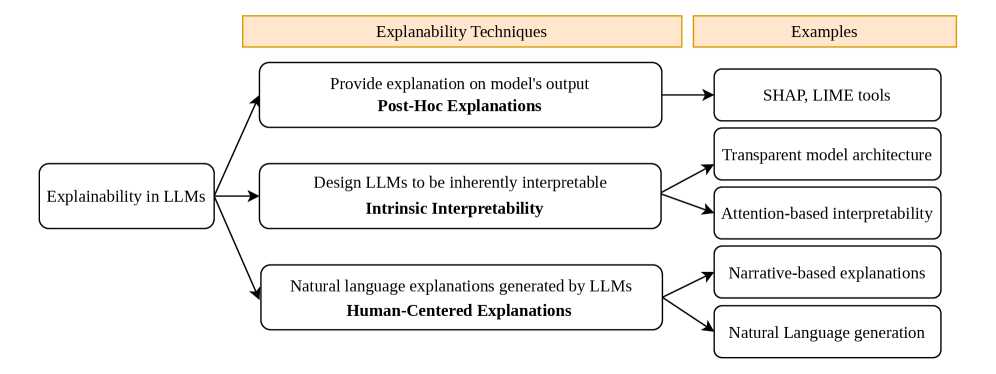
\includegraphics[width=0.9\linewidth]{img/xaicategories.png}
\caption{XAI Categories \cite{bilal_llms_2025}}
\label{fig:xai_categories}
\end{figure}
\paragraph{Post-hoc explanations}
Post-hoc explanations are generated after a model has produced its output and aim to explain that output by analysing the relationship between inputs and predictions. Rather than modifying the model itself, these methods treat the model as a fixed system and apply external analysis techniques to interpret its behaviour. Within this category, several subfamilies can be distinguished. 

\textbf{Gradient-based methods} such as SmoothGrad \cite{smilkov_smoothgrad_2017} and integrated gradients \cite{ancona_towards_2018} attribute output changes to input tokens by examining how the loss function responds to perturbations of the input signal. 

\textbf{Perturbation-based methods} such as SHAP (SHapley Additive exPlanations) \cite{lundberg_unified_2017} and LIME (Local Interpretable Model-agnostic Explanations)\cite{ribeiro_why_2016} assign importance scores to input features by systematically masking or modifying parts of the input and measuring the resulting change in output. 

\textbf{Decomposition-based methods} such as Layer-wise Relevance Propagation \cite{binder_layer-wise_2016} redistribute the model's output score back through the network layers to assign relevance to individual input components. 

\textbf{Surrogate-based methods} approximate a complex model locally with a simpler, interpretable model trained on perturbed samples. Together, these approaches have been extended to the token level for LLMs, allowing individual words or phrases to be highlighted as drivers of a model's output \cite{wu_usable_2025}.

\paragraph{Intrinsic interpretability}
Intrinsic interpretability refers to approaches that design or constrain the model itself to be inherently more transparent. 

One subclass consists of architectures built for transparency by design, such as Generalized Additive Models \cite{caruana_intelligible_2015}, Explainable Boosting Machines \cite{lou_accurate_2013}, and Interpretable Decision Sets \cite{lakkaraju_interpretable_2016}. However, these rule-based approaches are fundamentally incompatible with the dense, high-dimensional parameter spaces of neural networks and cannot be applied to LLMs without abandoning the representational capacity that makes such models effective. 

A second and practically more relevant subclass consists of \textbf{attention-based interpretability} methods, which examine the weights assigned by the model's self-attention mechanism to different parts of the input as a proxy for feature importance. 

A third subclass is \textbf{Chain-of-Thought (CoT) prompting}, which instructs the model to articulate its reasoning steps before arriving at a conclusion; insofar as the reasoning process is made visible as part of the model's own output, CoT can be understood as a form of intrinsic interpretability \cite{wu_usable_2025}.

\paragraph{Probing and mechanistic interpretability}
Probing and mechanistic interpretability methods represent a more technically ambitious strand that operates directly on the model's internal hidden-state representations rather than on its input-output behaviour. Probing classifiers attach lightweight diagnostic heads to intermediate layers to test what linguistic or factual properties are encoded at each depth of the network. 

More recent approaches such as SelfIE \cite{chen_selfie_2024} enable LLMs to interpret their own embeddings in natural language without additional training by injecting a hidden state of interest into a secondary forward pass; such methods are structurally grounded in the model's actual internal representations rather than its output text. However, they require white-box access to model weights and remain largely opaque to non-technical audiences.

\paragraph{Human-centred and narrative explanations}
Human-centred and narrative explanations are natural language explanations generated by LLMs themselves, either through self-explanation or through the use of a separate model tasked with explaining the outputs of another \cite{bilal_llms_2025}. These include narrative-based explanations and approaches that leverage the language generation capabilities of LLMs to produce accessible, user-friendly accounts of model behaviour. 

A notable subclass are \textbf{counterfactual explanations}, which characterize a model's decision boundary by describing the minimal change to an input that would alter the output \cite{wachter_counterfactual_2018}; extensions of this idea have moved beyond single-feature perturbations toward actionable, multistep recourse paths \cite{rawal_beyond_2020}. 

A related line of work explores \textbf{gamification frameworks} that use narrative and interactive presentation to increase engagement with explanations among lay users \cite{you_gamifying_2024}. The central challenge across this entire category is that the generated explanation is itself an LLM output and therefore subject to the same reliability and faithfulness limitations as the original response.

\textbf{Uncertainty quantification} constitutes a further dimension of XAI that cuts across the categories above. Methods in this class communicate the model's estimated confidence in its output, either through calibrated probability scores derived from token-level log-probability distributions or through hedged natural language formulations. Aligning expressed confidence with actual response quality is a non-trivial problem, and miscalibrated confidence can lead users to over-trust or under-trust model outputs \cite{tao_when_2024}.

\textbf{Human-AI Collaboration (HAIC) frameworks} represent an emerging category that extends the scope of XAI beyond individual explanation methods toward the broader sociotechnical context of human-AI interaction \cite{jeong_design_2025}. Frameworks such as Human-in-the-Loop (HITL) and Human-on-the-Loop (HOTL) position the user as an active participant in AI-assisted decision-making, foregrounding the need for tools that help users maintain appropriate oversight rather than simply delegating judgment to the model. This perspective emphasizes that effective explainability depends not only on the technical properties of a given method but also on mutual understanding, appropriate role allocation, and calibrated trust between the human and the system.

A notable gap that persists across all of these categories is that most XAI research focuses on technical audiences. There is limited empirical evidence on which explanation types are most effective for lay users interacting with LLMs in everyday contexts \cite{wu_usable_2025}.

\subsection{Selected XAI Methods}
\label{sec:selected_xai_methods}

Based on the taxonomy described above, three methods were selected for this study, each representing a distinct explanation paradigm: post-hoc attribution (SHAP), process transparency (Chain-of-Thought), and uncertainty quantification (confidence indication). The selection criteria were: coverage of distinct explanation paradigms, feasibility of implementation, and accessibility to non-expert users.

\textbf{SHAP and Counterfactual Reasoning} represent the post-hoc explanation category. SHAP is grounded in Shapley values from cooperative game theory \cite{lundberg_unified_2017}. It decomposes a model's output into contributions attributable to each input feature, providing a principled and consistent attribution method. In this study, SHAP is applied at the token level to highlight which parts of a prompt most strongly influenced the model's response. This is complemented by counterfactual reasoning, which presents users with a modified version of the input alongside the resulting change in output, offering an intuitive causal account of model behaviour.

\textbf{Chain-of-Thought (CoT) prompting} represents the intrinsic interpretability category. By including an explicit instruction in the system prompt for the model to reason through its answer step by step before providing a conclusion, CoT makes the model's intermediate reasoning visible as part of the response itself. This approach requires no post-hoc analysis and produces explanations in natural language, making it particularly suited to lay audiences \cite{wu_usable_2025}.

\textbf{Confidence indication} represents the uncertainty quantification dimension of XAI. Confidence scores communicate the model's estimated certainty in its output, either derived from token-level probability distributions or expressed through calibrated natural language hedging. Research suggests that aligning expressed confidence with actual response quality is a non-trivial problem, and that miscalibrated confidence can lead users to over-trust or under-trust model outputs \cite{tao_when_2024}. Including this method allows the study to examine whether explicit uncertainty communication affects user trust independently of the content of the explanation.

\section{Trust in AI Systems}

\subsection{Defining Trust}
\label{sec:trust_theory}

Trust is a multidimensional construct that has been studied across philosophy, cognitive science, and human-computer interaction. At its core, trust involves a willingness to accept vulnerability based on positive expectations about another agent's behaviour \cite{jones_concept_2002}. In the context of AI systems, trust can be understood as a user's disposition to rely on the system's outputs, shaped by beliefs about the system's competence, reliability, and intentions \cite{falcone_social_2001}.

For the purposes of this study, the operationalisation of trust draws on a framework that distinguishes four theoretical dimensions \cite{jones_concept_2002, falcone_social_2001, castelfranchi_trust_2001}: trust in the environment and the sociotechnical infrastructure in which the system operates, trust in the AI agent itself and any mediating agents involved in producing its outputs, trust in the system as an interaction partner, and trust in the system as an authoritative source of information. These dimensions together capture the layered nature of the trust relationship between a user and an LLM, spanning infrastructure-level reliability, agent-level competence and intention, and the social and epistemic weight a user assigns to the system's outputs. From this theoretical foundation, five sentences describing these four aspects were derived as a measurement instrument for use in the empirical study, which is described in detail in Section~\ref{sec:trust_instrument}.

\subsection{Trust in the Context of LLMs}
\label{sec:trust_in_context_of_llms}

The fluency and apparent confidence of LLM outputs creates a particular risk of miscalibrated trust. Users who are not familiar with the failure modes of LLMs may attribute a level of reliability to model outputs that is not warranted by the model's actual accuracy \cite{schwartz_enhancing_2023}. Conversely, users who become aware of hallucination through negative experiences may develop excessive scepticism that prevents them from benefiting from the model's genuine capabilities.

Research on sycophancy in LLMs illustrates a further complication: models trained to be agreeable and conversationally pleasant may produce outputs that increase user trust precisely by telling users what they want to hear, independent of factual accuracy \cite{sun_be_2026}. This dynamic makes it especially important to develop tools that help users form well-grounded assessments of model reliability rather than relying on surface features of the interaction such as fluency or tone.

XAI methods represent one promising avenue for supporting better-calibrated trust. By making aspects of model behaviour visible, such as which inputs drove a response, how certain the model is, or what reasoning it followed, XAI has the potential to help users identify outputs that warrant closer scrutiny. Whether this potential is realized in practice, and which explanation types are most effective for general users, remains an open empirical question that this study addresses.

\subsection{Addressing Trust Through XAI Methods}

\begin{wrapfigure}{R}{0.4\textwidth}
    \centering
    \vspace{-\baselineskip}
    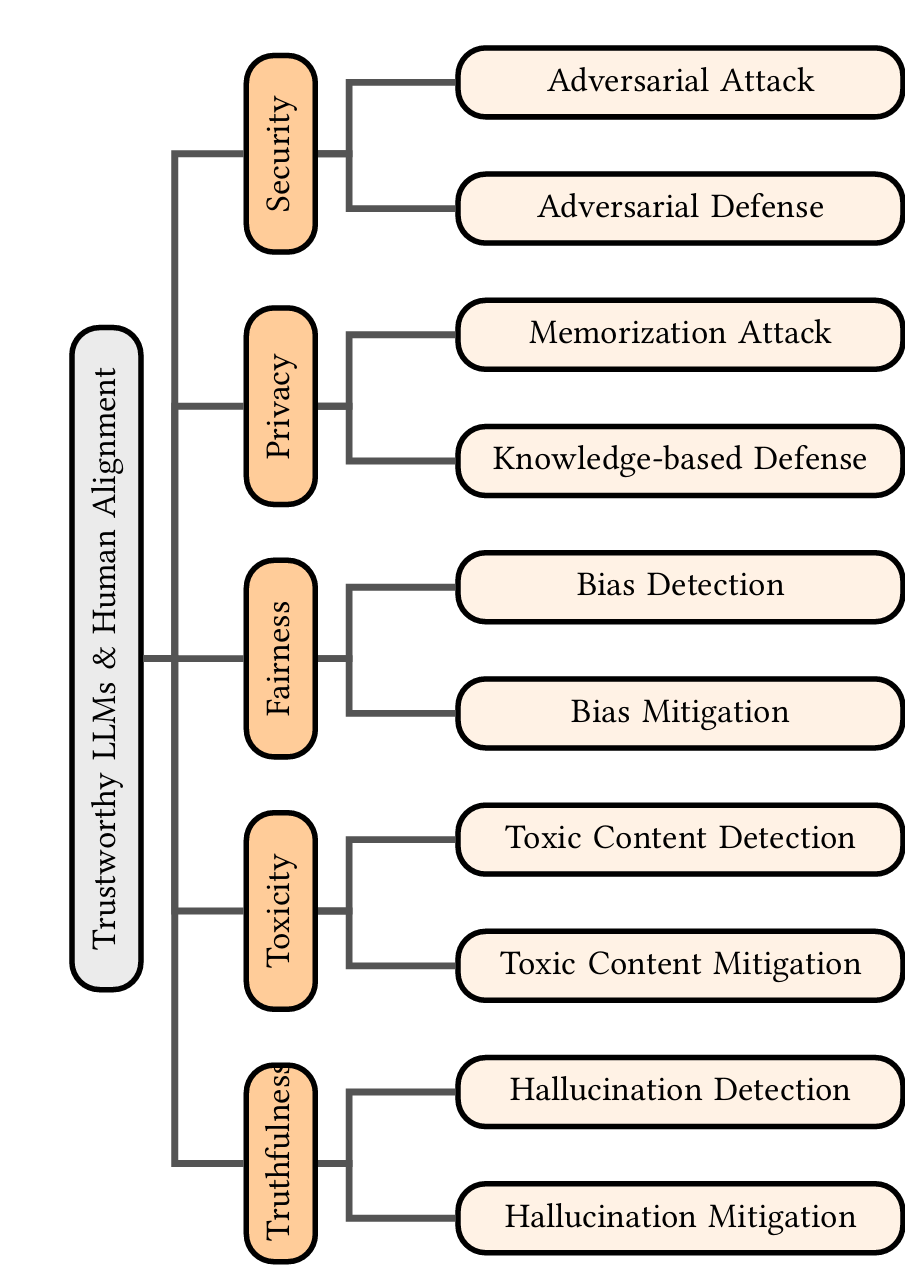
\includegraphics[width=\linewidth]{img/trustworthynessExplanations.png}
    \caption{Taxonomy of explanation techniques for trust\-worthi\-ness aspects of LLMs \cite{wu_usable_2025}}
    \vspace{-0.2cm}
    \label{fig:xaiTrustworthyness}
\end{wrapfigure}

As illustrated in Figure~\ref{fig:xaiTrustworthyness}, the taxonomy proposed in \cite{wu_usable_2025} maps explainability techniques to specific trustworthiness dimensions of LLMs, including security, privacy, fairness, toxicity, and truthfulness. This mapping provides a principled basis for selecting XAI methods that target the trust concerns most relevant to lay users interacting with general-purpose LLMs.

The three methods selected for this study each address distinct dimensions of the trust relationship described in Section~\ref{sec:trust_theory}. SHAP-based attribution and counterfactual reasoning target trust at the level of the AI agent and its outputs: by making visible which parts of a prompt drove a given response, and by illustrating how alternative inputs would have changed that response, these methods support the user's ability to assess the reliability and competence of the system. They are particularly suited to addressing concerns about hallucination and ungrounded outputs, where users benefit from understanding the evidential basis of a response \cite{wu_usable_2025}.

Chain-of-Thought prompting addresses trust at the level of the system as an interaction partner. By externalizing the model's intermediate reasoning steps, CoT makes the inferential process legible and allows users to identify where a reasoning chain may have gone astray. This approach aligns with the intrinsic interpretability category of XAI and supports calibrated trust by providing users with a basis for evaluating the plausibility of the model's conclusions rather than accepting them on the basis of surface fluency alone \cite{wu_usable_2025}.

Confidence indication addresses the epistemic dimension of trust, namely the degree to which users treat the system as an authoritative source of information. Explicitly communicating the model's uncertainty, whether through calibrated probability scores or hedged natural language formulations, provides users with a direct signal that can modulate reliance. Research suggests that this dimension is particularly important given the tendency of LLMs to produce fluent but overconfident outputs that can mislead users who lack the domain knowledge to independently verify claims \cite{tao_when_2024}.

Together, these three methods offer complementary coverage of the trust dimensions identified in the theoretical framework, and their differential effects on user trust constitute the primary empirical question of this study.